\section{Question 1: Unimolecular decay}

In this part of the question, 
only the decay processes are considered. 
The decay process is modeled as a two-state, 
continuous-time process, with $state_1$ as undecayed state 
and $state_0$ as a decayed state.

\subsection{Graph and Rate Matrix}

The Figure \ref{fig:state_graph} represent the transfer of between
two states 
and the rate matrix is stated in equation \ref{eq:rate_matrix}.

\begin{minipage}{.5\textwidth}
\includegraphics[width=\linewidth]{img/figure1.png}
\captionof{figure}{Transition Graph}
\label{fig:state_graph}
\end{minipage}
\begin{minipage}{.5\textwidth}
    \begin{equation}
        \mathbf{K} = \begin{pmatrix}
            0 & \nu \\
            0 & -\nu
            \end{pmatrix}
        \label{eq:rate_matrix}
    \end{equation} 
\end{minipage}

\subsection{Obtain $p_0(t)$ }
Master Equation (equation \ref{eq:Master_equation}) 
can be obtained by substituting the rate matrix
(equation \ref{eq:rate_matrix}) in it.
Since the state either be $state_1$ or $state_0$
($p_1(t) + p_0(t) = 1$),
$p_1(t) = 1 - p_0(t)$.
Using this information to subsitude $p_1(t)$ 
and $p_0(t)$ can be solved.

\begin{equation}
    \frac{d}{dt}
\begin{pmatrix}
p_0(t) \\
p_1(t)
\end{pmatrix}
= \mathbf{K}
\begin{bmatrix}
p_0(t) \\
p_1(t)
\end{bmatrix}
= \begin{pmatrix}
    0 & \nu \\
    0 & -\nu
    \end{pmatrix}
    \begin{bmatrix}
        p_0(t) \\
        p_1(t)
        \end{bmatrix}  
\label{eq:Master_equation}
\end{equation}

\begin{align*}
    \frac{d p_0(t)}{dt} &= \nu p_1 = \nu (1 - p_0(t)), \quad
    \frac{1}{1 - p_0(t)} dp_0(t) = \nu dt , \quad
    \int \frac{1}{1 - p_0(t)} dp_0(t) = \int \nu dt \\
    -\ln |1 - p_0(t)| &= \nu t + C , \quad
    |1 - p_0(t)| = e^{-\nu t - C} ,\quad
    1 - p_0(t) = \pm e^{-C} e^{-\nu t} \\
    p_0(t) &= 1 - C' e^{-\nu t}, \quad
    \because p_0(0) = 0, \quad
    \therefore 0 = 1 - C', C' = 1\\
    p_0(t) &= 1 - e^{-\nu t}
\end{align*}

\subsection{Distribution of Decay Times}
To obtain the distribution of decay time ($p(t_{\text{dec}})$), 
a relationship between $p_0(t)$ and $p(t_{\text{dec}})$ 
could be found and used to solve $p(t_{\text{dec}})$, 
since $p_0(t)$ already be calculated.

\begin{align*}
    \because p(t_{\text{dec}}) \delta t_{\text{dec}} &= 
    p_0(t_{\text{dec}} + \delta t_{\text{dec}}) - p_0(t_{\text{dec}})
    = p_0(t_{\text{dec}}) + \frac{d}{d t_{\text{dec}}}p_0(t_{\text{dec}})\delta t_{\text{dec}} - p_0(t_{\text{dec}}) \: (\text{Taylor Expansion})\\
    \therefore p(t_{\text{dec}}) &= \frac{d}{d t_{\text{dec}}}p_0(t_{\text{dec}})
    = \frac{d}{d t_{\text{dec}}}(1 - e^{-\nu t_{\text{dec}}})
    = \nu e^{-\nu t_{\text{dec}}}
\end{align*}

\subsection{Mean and Variance of Decay Time}
Mean($\langle T_{\text{dec}} \rangle$) and variance ($\text{VAR}(T_{\text{dec}})$) can be 
calculated by equation \ref{eq:mean_Variance}.

\begin{equation}
    \langle T_{\text{dec}} \rangle = \int_{0}^{\infty} t_{\text{dec}} \cdot p(t_{\text{dec}}) \, dt_{\text{dec}}, \quad
    \text{VAR}(T_{\text{dec}}) = \int_{0}^{\infty} (t_{\text{dec}} - \langle T_{\text{dec}} \rangle)^2 \cdot p(t_{\text{dec}}) \, dt_{\text{dec}}
    \label{eq:mean_Variance}
\end{equation}

\begin{align*}
    \langle T_{\text{dec}} \rangle &= \int_{0}^{\infty} t_{\text{dec}} \cdot p(t_{\text{dec}}) \, dt _{\text{dec}}
    = \int_{0}^{\infty} t_{\text{dec}} \cdot \nu e^{-\nu t_{\text{dec}}} \, dt_{\text{dec}}
    = \nu \int_{0}^{\infty} t_{\text{dec}} \cdot e^{-\nu t_{\text{dec}}} \, dt_{\text{dec}}\\
    &= \nu(- \frac{t_{\text{dec}} e^{-\nu t_{\text{dec}}}}{\nu} \bigg|_0^{\infty} + \int_{0}^{\infty} \frac{1}{\nu} e^{-\nu t_{\text{dec}}} dt_{\text{dec}})
    = - t_{\text{dec}} e^{-\nu t_{\text{dec}}} \bigg|_0^{\infty} + \int_{0}^{\infty} e^{-\nu t_{\text{dec}}} dt_{\text{dec}}\\
    &= \int_{0}^{\infty} e^{-\nu t_{\text{dec}}} dt_{\text{dec}} = -\frac{1}{\nu} e^{-\nu t_{\text{dec}}}\bigg|_0^{\infty}=\frac{1}{\nu}\\
    \text{VAR}(T_{\text{dec}}) &= \int_{0}^{\infty} (t_{\text{dec}} - \langle T_{\text{dec}} \rangle)^2 \cdot p(t_{\text{dec}}) \, dt_{\text{dec}}
    = \nu \int_{0}^{\infty} (t_{\text{dec}} - \frac{1}{\nu})^2 \cdot e^{-\nu t_{\text{dec}}} \, dt_{\text{dec}}\\
    &= \nu \int_{0}^{\infty} (t_{\text{dec}}^2 - \frac{2 t_{\text{dec}}}{\nu} + \frac{1}{\nu^2}) \cdot e^{-\nu t_{\text{dec}}} \, dt_{\text{dec}}\\
    &= \nu \int_{0}^{\infty} t_{\text{dec}}^2 e^{-\nu t_{\text{dec}}} dt_{\text{dec}} - 2 \int_{0}^{\infty} {t_{\text{dec}}}  e^{-\nu t_{\text{dec}}} dt_{\text{dec}} + \frac{1}{\nu} \int_{0}^{\infty} e^{-\nu t_{\text{dec}}} dt_{\text{dec}}\\
    &= \nu \int_{0}^{\infty} t_{\text{dec}}^2 e^{-\nu t_{\text{dec}}} dt_{\text{dec}} - \frac{2}{\nu^2} + \frac{1}{\nu^2}
    = \nu \int_{0}^{\infty} t_{\text{dec}}^2 e^{-\nu t_{\text{dec}}} dt_{\text{dec}} - \frac{1}{\nu^2}\\
    &=\nu\left( - \frac{t_{\text{dec}}^2}{\nu} e^{-\nu t_{\text{dec}}} \bigg|_{0}^{\infty} + \int_{0}^{\infty} \frac{2t_{\text{dec}}}{\nu} e^{-\nu t_{\text{dec}}} dt_{\text{dec}} \right)- \frac{1}{\nu^2}\\
    &= \nu \left(0 +  \frac{2}{\nu^3} \right) - \frac{1}{\nu^2} = \frac{1}{\nu^2}
\end{align*}

\section{Question 2: Diffusion}

\subsection{Free Diffusion in an Infinite System}

To verify whether equation \ref{eq:solution} is the solution
of equation \ref{eq:equation}, 
only need to substitute equation \ref{eq:solution} back to 
equation \ref{eq:equation}.


\begin{minipage}{.5\textwidth}
    \begin{equation}
        q(x, t) = \sqrt{\frac{1}{4\pi Dt}} \, e^{-\frac{(x - \frac{L}{2})^2}{4Dt}}
        \label{eq:solution}
    \end{equation}
\end{minipage}
\begin{minipage}{.5\textwidth}
    \begin{equation}
        \frac{\partial q(x, t)}{\partial t} = D \frac{\partial^2 q(x, t)}{\partial x^2}
        \label{eq:equation}
    \end{equation}
\end{minipage}
\begin{align*}
    \text{Set} \: A(t) &= \sqrt{\frac{1}{4\pi Dt}}, \, B(t) = e^{-\frac{(x - \frac{L}{2})^2}{4Dt}}
    \text{and} \: A'(t) = - \frac{1}{4 \sqrt{\pi D} t^{\frac{3}{2}}}, \, 
    B'(t) = \frac{\left(- \frac{L}{2} + x\right)^{2} e^{- \frac{\left(- \frac{L}{2} + x\right)^{2}}{4 D t}}}{4 D t^{2}}\\
    \frac{\partial q(x, t)}{\partial t} &= A'(t) \cdot B(t) + B'(t) \cdot A(t)
    = - \frac{1}{4 \sqrt{\pi D} t^{\frac{3}{2}}} \cdot e^{-\frac{(x - \frac{L}{2})^2}{4Dt}} + 
    \frac{\left(- \frac{L}{2} + x\right)^{2} e^{- \frac{\left(- \frac{L}{2} + x\right)^{2}}{4 D t}}}{4 D t^{2}} \cdot \sqrt{\frac{1}{4\pi Dt}}\\
    \frac{\partial q}{\partial t} &= -\frac{B(t)}{4\sqrt{\pi D} t^{\frac{3}{2}}} + \frac{(x - \frac{L}{2})^2 B(t)}{8\sqrt{\pi} D^{\frac{3}{2}} t^{\frac{5}{2}}}
    = \left(\frac{(2x - L)^2 - 8Dt}{16Dt^2}  \right) \cdot \frac{B(t)}{\sqrt{4 \pi D t}}\\
    \text{Set} \: C(x) &= e^{-\frac{(x - \frac{L}{2})^2}{4Dt}}, \, C'(x) = \frac{(L - 2 x) C(x)}{4 D t}, \, E = \sqrt{\frac{1}{4\pi Dt}}\\
\end{align*}

\begin{align*}
    \frac{\partial q(x, t)}{\partial x} &= E \cdot C'(x), \quad
    \frac{\partial^2 q(x, t)}{\partial x^2} =\frac{\partial}{\partial x} \left[ \frac{E}{4Dt} \cdot (L-2x) \cdot C(x) \right]
    = \frac{E}{4Dt} \cdot \frac{\partial}{\partial x} \left[(L-2x) \cdot C(x) \right]\\
    \frac{\partial}{\partial x} &\left[(L-2x) \cdot C(x) \right] = L \cdot C'(x) - 2 \frac{\partial}{\partial x}[x\cdot C(x)] , \quad
    \frac{\partial}{\partial x}[x\cdot C(x)] = C(x) + x C'(x)\\
    \frac{\partial^2 q(x, t)}{\partial x^2} &= \frac{E}{4Dt} \cdot [L \cdot C'(x) - 2 \cdot C(x) - 2x\cdot C'(x)]
    = \frac{E}{4Dt} [(L-2x)C'(x) - 2C(x)]\\
    &= \frac{E}{4Dt} \left[\frac{(L-2x)^2 C(x)}{4Dt} - 2C(x)\right]
    = \frac{E}{4Dt} \left[\frac{(L-2x)^2}{4Dt} - 2\right] \cdot C(x)\\
    &= \frac{E}{4Dt} \left[\frac{(L-2x)^2 - 8Dt}{4Dt}\right] \cdot C(x)
    = \frac{(L-2x)^2 - 8Dt}{16D^2t^2} \cdot \frac{C(x)}{\sqrt{{4\pi Dt}}}\\
    &\because C(x) = B(t) \, \text{(They are the same fucntion, just fix different variable)}\\
    &\therefore \frac{(L-2x)^2 - 8Dt}{16D^2t^2} \cdot \frac{C(x)}{\sqrt{{4\pi Dt}}} = D \cdot \frac{(2x - L)^2 - 8Dt}{16Dt^2} \cdot \frac{B(t)}{\sqrt{4 \pi D t}}\\
    & \quad \frac{\partial q(x, t)}{\partial t} = D \frac{\partial^2 q(x, t)}{\partial x^2}
\end{align*}

\subsection{Find $Q^{\infty}(t)$}
$Q^{\infty}(t)$ is the probability that the position of the 
protein outside the region($0<x<L$).
Therefore, $Q^{\infty}(t) = \int_{-\infty}^{0} q(x,t)dx + \int_{L}^{+ \infty} q(x,t)dx$. 


\subsection{Multiply Choise Question}

Option 1 is the correct one. 
Since if one protein is outside of the axon, 
it means it must have reached $x=L$ or $x=0$. 
However, 
if one protein, 
has reached the $x=L$ or $x=0$, 
it is not necessarily outside the axon. 
Since one protein may have reached 
the $x=L$ or $x=0$ and then diffused back into the axon. 

\subsection{Using simulation to estimate PDF}

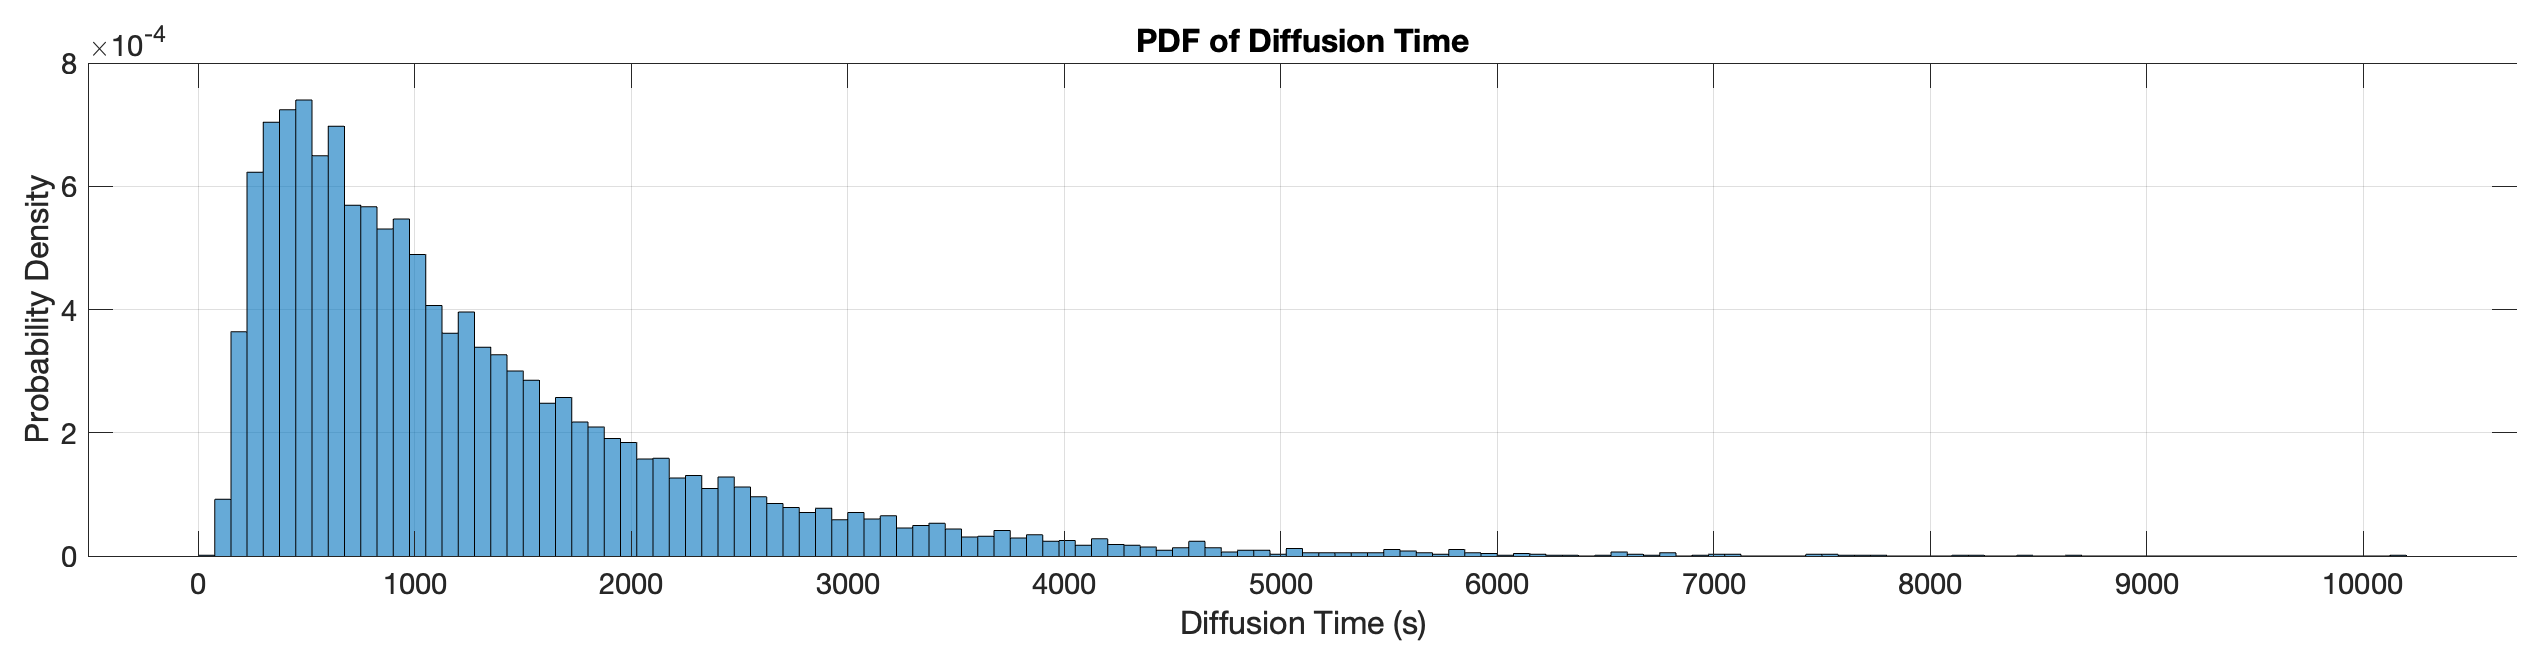
\includegraphics[width=\linewidth]{img/figure2.eps}
\captionof{figure}{PDF for Diffusion Time}
\label{fig:q2.4}

The code that generates this figure can be found in the appendix.


\subsection{Calculate $\langle T_{diff} \rangle$ and $\text{VAR}(T_{\text{diff}}) $}

$\langle T_{diff} \rangle$ and $Var(T_{diff} )$ is calculated 
by the simulation data generated in the last section. 
The $\langle T_{diff} \rangle$ is equal to 1261, 
and $\text{VAR}(T_{\text{diff}}) $ is equal to 1069503.4.

\section{Question 3: Comparing decay and diffusion}

\subsection{$\nu$ for $\langle T_{dec} \rangle =  \langle T_{diff} \rangle$}

$\langle T_{dec} \rangle$ is already calculated in question 1.4, 
that is $\langle T_{dec} \rangle = \frac{1}{\nu}$. 
$\langle T_{diff} \rangle$ is also calculated in 
question 2.5, 
which is $\langle T_{diff} \rangle = 1261$.
If $\nu$ for $\langle T_{dec} \rangle =  \langle T_{diff} \rangle$, 
then $\frac{1}{\nu} = 1261$. 
$\nu = \frac{1}{1261}$. 

Since $p(t_{dec})$ is already calculated, 
substitute $\nu = \frac{1}{1261}$ can get a 
PDF which is demonstrated by 
blue line in figure \ref{fig:q3.1}, 
and the distribution of diffusion is calculated from 
data generated from section 2.4, 
and estimate the PDF distribution 
by function $\mathtt{ksdensity}$.

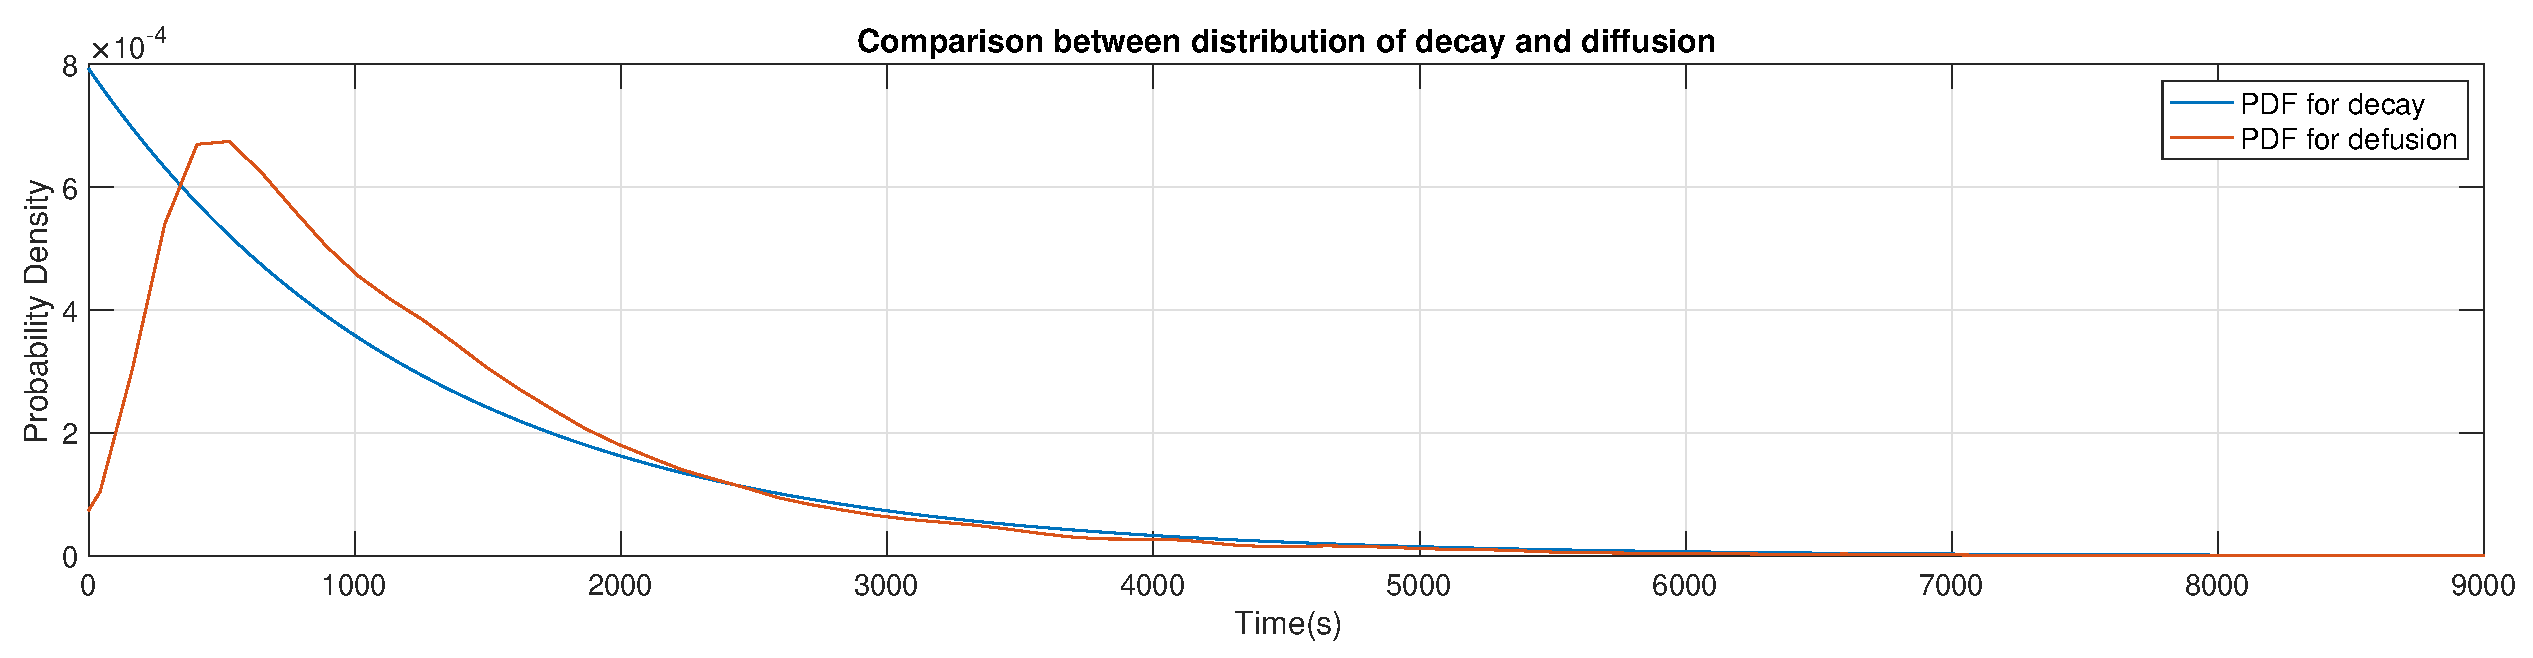
\includegraphics[width=\linewidth]{img/figure3.eps}
\captionof{figure}{Comparison between the distribution of decay and diffusion}
\label{fig:q3.1}

The $\text{VAR}(T_{\text{dec}})$ can also be 
calculated, 
assuming $\langle T_{dec} \rangle =  \langle T_{diff} \rangle$, 
and $\nu = \frac{1}{1261}$. 
$\text{VAR}(T_{\text{dec}}) = \frac{1}{\nu^2}$, 
calculated in section 1.4, 
and it is equal to $1261^2 = 1590121$. 
It is bigger than $\text{VAR}(T_{\text{diff}}) $, 
which is calculated in section 2.5, 
it is equal to $1069503.4$.

$\therefore \text{VAR}(T_{\text{dec}}) > \text{VAR}(T_{\text{diff}})$


\subsection{Short Times Event}

If $\langle T_{dec} \rangle =  \langle T_{diff} \rangle = 1261$, 
then $\frac{1}{10} \langle T_{dec} \rangle = \frac{1}{10} \langle T_{diff} \rangle = 126.1$. 
Based on figure \ref{fig:q3.1}, 
$p(126.1) > q(126.1)$. 
It means if there is an event happened, 
it is more possible this event is a decay 
than diffusion out of the main body.


This can be explained by the physics 
behind decay and diffusion.
Decay can happen instantly, 
therefore, it has an exponential decay 
of the probability against time. 
However, 
it normally takes some for a protein to diffuse 
to somewhere, 
thus, 
diffusion has a positively skewed distribution. 
This explained why in a short time, 
a event happened it is more possible 
because of decay rather than diffusion.

\subsection{Decay occurs before Diffuse outside}
The probability of 
decay event happened before 
protein diffuse outside of the axon 
is about 0.54, 
this result is calculated by taking the mean 
of multiple simulation results.
(more detailed code is shown in the appendix)

\subsection{$\langle T_{diff,new} \rangle$ and $\langle T_{diff,new} \rangle$}

If considering only decay events that happen before diffusion 
out of the axon, 
the new $\langle T_{dec} \rangle$ will smaller 
than original $\langle T_{dec} \rangle$,  
and if only considering 
the diffusion events that happen before decay, 
new $\langle T_{diff} \rangle$ is also smaller  
than original $\langle T_{diff} \rangle$. 
This result is generated by multiply 
$\mathtt{Matlab}$ simulation(detailed code is in the appendix).
\newpage